\begin{tikzpicture}
	\node (S1) at (-1.5,-3.5) {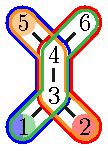
\includegraphics[scale=.8]{starSparseS1}};
	\node (S2) at (1.5,-3.5) {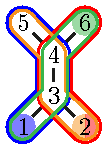
\includegraphics[scale=.8]{starSparseS2}};
	\node (T1) at (-1.5,3.5) {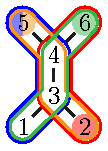
\includegraphics[scale=.8]{starSparseT1}};
	\node (T2) at (1.5,3.5) {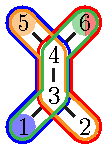
\includegraphics[scale=.8]{starSparseT2}};
	\node (S) at (0,.5) {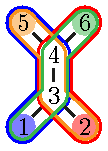
\includegraphics[scale=.8]{starSparseS}};
	\node (sigma1) at (-1.5,-2.3) {$152634$};
	\node (sigma2) at (1.5,-2.3) {$261534$};
	\node (tau1) at (-1.5,2.3) {$526134$};
	\node (tau2) at (1.5,2.3) {$615234$};
	\node[draw,circle,inner sep=1] at (-2.2,-3.5) {$S_1$};
	\node[draw,circle,inner sep=1] at (2.2,-3.5) {$S_2$};
	\node[draw,circle,inner sep=1] at (-2.2,3.5) {$T_1$};
	\node[draw,circle,inner sep=1] at (2.2,3.5) {$T_2$};
	\node[draw,circle,inner sep=1] at (.6,.5) {$S$};
%	\draw (sigma1.north) -- (S.south west);
%	\draw (sigma2.north) -- (S.south east);
%	\draw (S.north west) -- (tau1.south);
%	\draw (S.north east) -- (tau2.south);
	\draw (sigma1.north) -- (tau1.south);
	\draw (sigma1.north) edge [bend right] (tau2.south);
	\draw (sigma2.north) edge [bend left] (tau1.south);
	\draw (sigma2.north) -- (tau2.south);
\end{tikzpicture}
